\chapter{Discussion and results}
\section{Discussion}
\section{Recommendations for future work}



\subsection{Multithreading}
If a function blocks the execution of our single thread, the whole program runs slower, which in turn leads to an increased delay in the control system and may make the auto tracking CCTV system unstable.

By separating functionality into threads that run by themselves and communicate using ZeroMQ or similar software library, a temporary latency spike in the communication between a camera and the software will not slow down the rest of the system.

In order to implement this fully, great care needs to  be taken to ensure that either we wait for all data to be present before we act upon it, or we discard it if it gets delayed too much to ensure a near-realtime behavior.

\begin{figure}[ht]
    \centering
    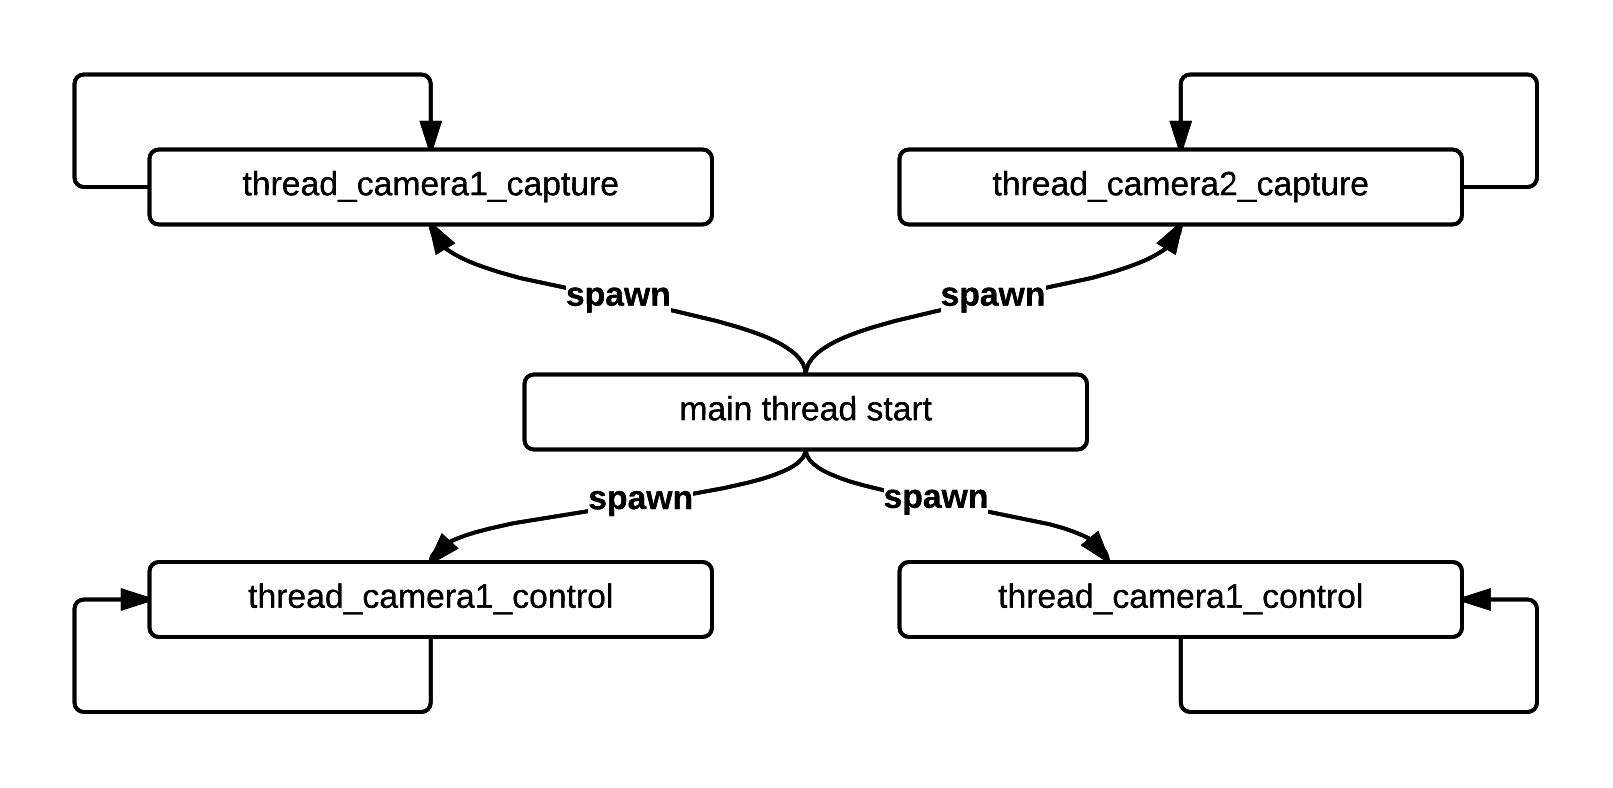
\includegraphics[width=1.0\textwidth]{software_multithread.png}
    \caption{Multithreading concept runs camera capture independent of camera PTZ control. Source: Own work}
    \label{fig:software_multithread}
\end{figure}
\FloatBarrier

\subsection{Augmented Reality}
In order to provide the driller and assistant driller with valuable information, a heads-up display could be used. This could use the video stream from the auto tracking CCTV cameras to overlay useful information depending on where in a sequence the machines are. By augmenting the image with data from both the control system as well as data interpreted from the machine vision system, we may also use data fusion to determine how accurate the displayed data is, and output the best result possible.

\begin{figure}[ht]
    \centering
    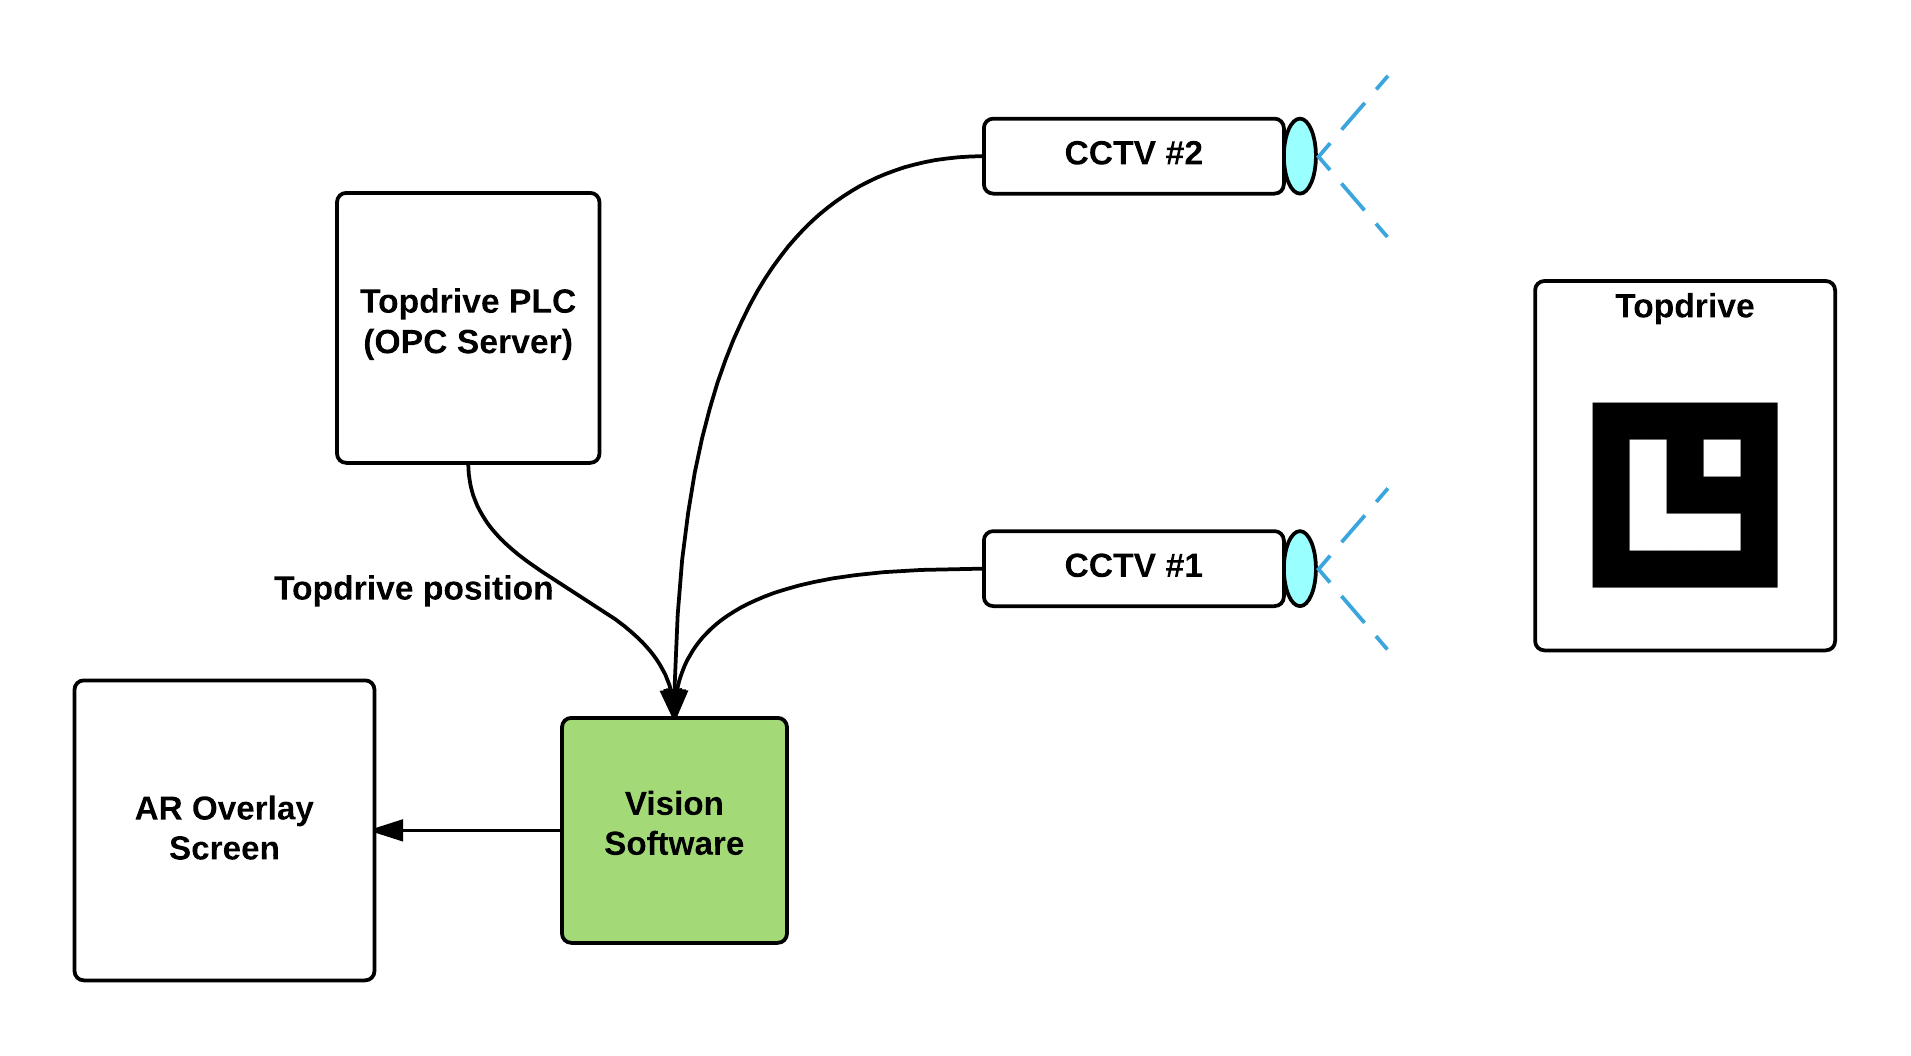
\includegraphics[width=1.0\textwidth]{augmented_data_flow.png}
    \caption{Data fusion using PLC and vision data. Source: Own work}
    \label{fig:augmented_data_flow}
\end{figure}
\FloatBarrier


\begin{figure}[ht]
    \centering
    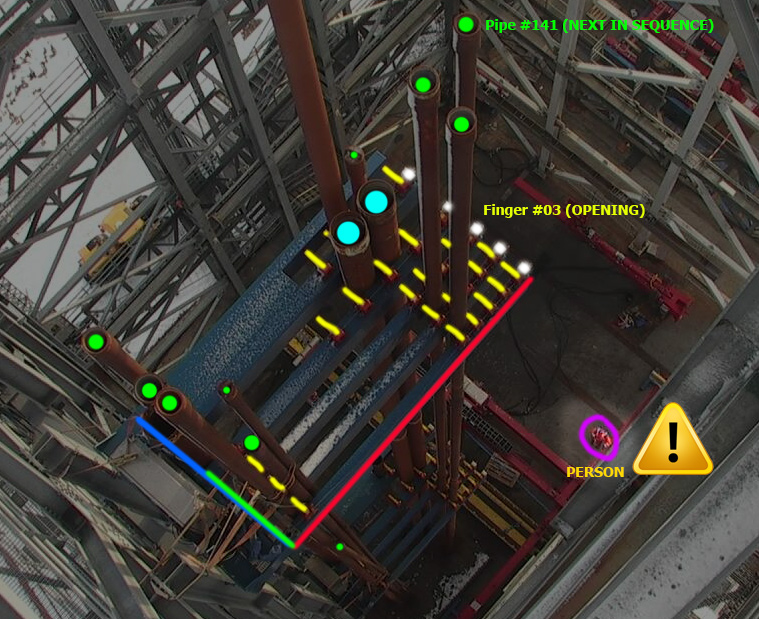
\includegraphics[width=1.0\textwidth]{mockup_augmented_reality.jpg}
    \caption{Fingerboard augmented reality mockup. Source: Own work}
    \label{fig:mockup_augmented_reality}
\end{figure}
\FloatBarrier

\begin{figure}[ht]
    \centering
    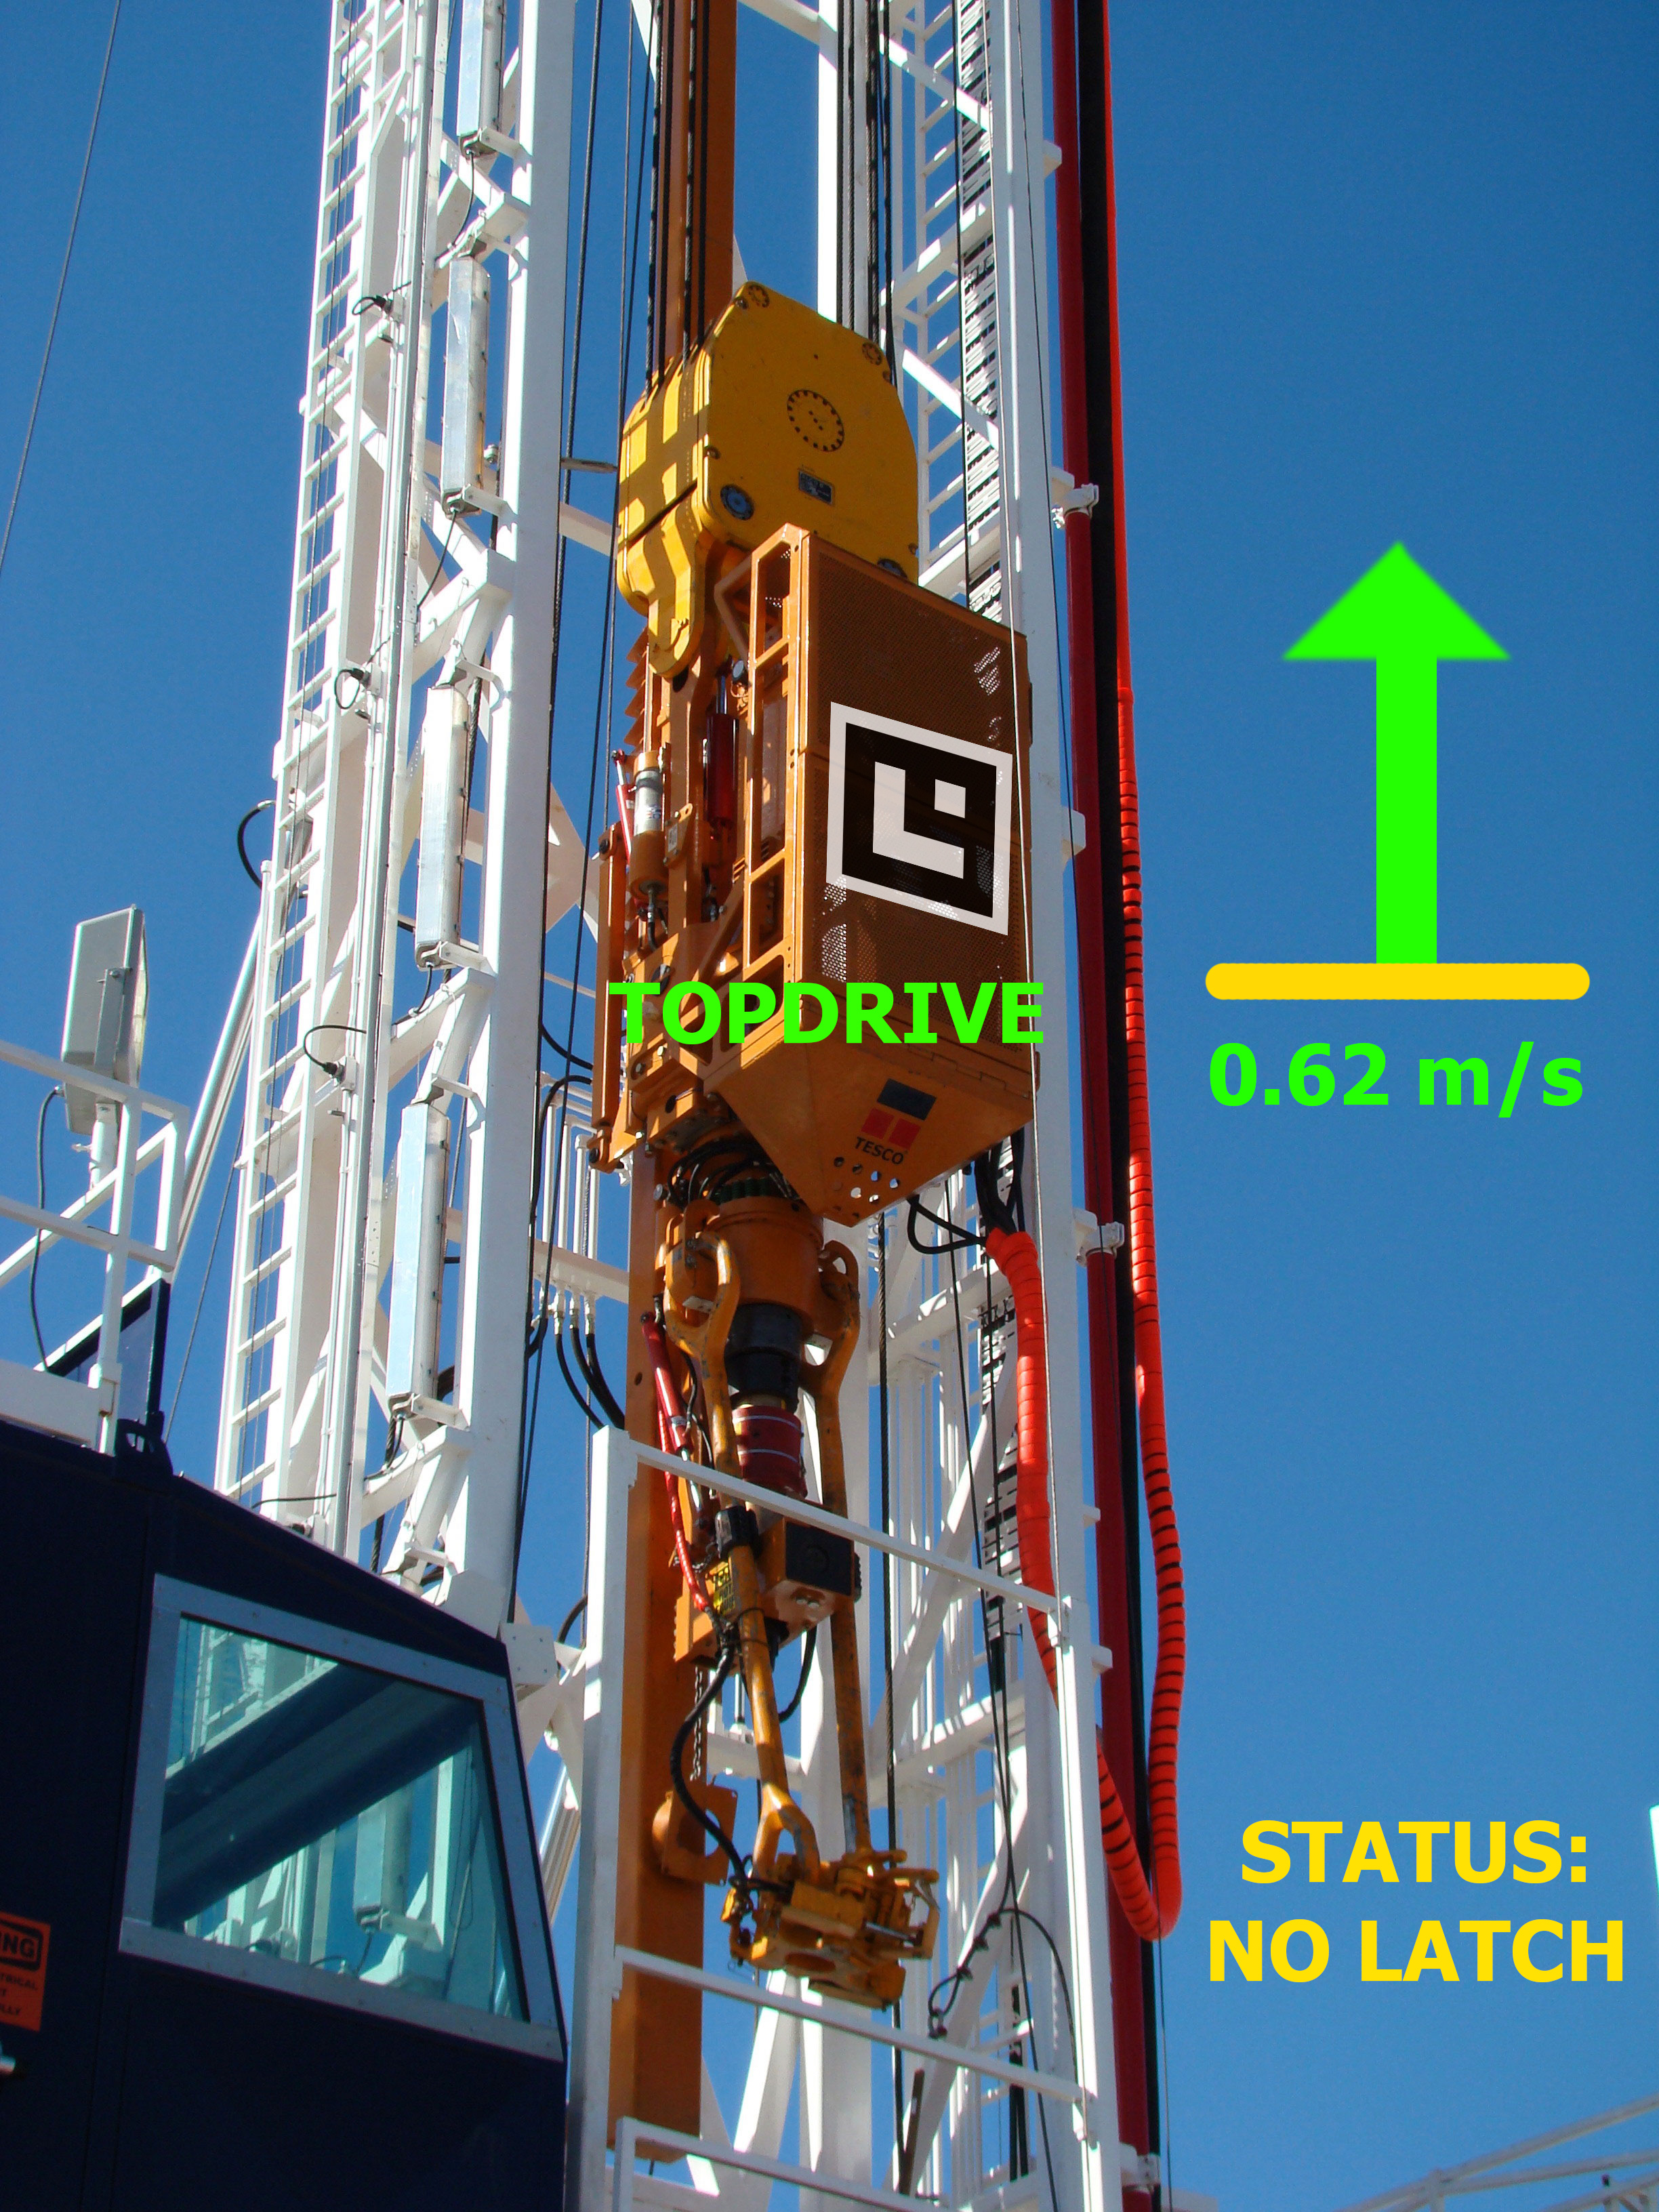
\includegraphics[width=0.8\textwidth]{mockup_augmented_reality_topdrive.jpg}
    \caption{Topdrive augmented reality mockup. Source: \citet{dc15} modified by author}
    \label{fig:mockup_augmented_reality_topdrive}
\end{figure}
\FloatBarrier